\setcounter{page}{1}

\section{Introducción}
    Ejemplo de cita~(\cite{buffett84}).
\section{Objetivos}
    \begin{itemize}
        \item Emplear PAT en la interacción de redes privadas - redes públicas.
    \end{itemize}

\section{Desarrollo del Trabajo}
    \subsection{Topología}
    Para esta práctica utilizaremos la siguiente topología.
    \begin{figure}[H]
        \centering
        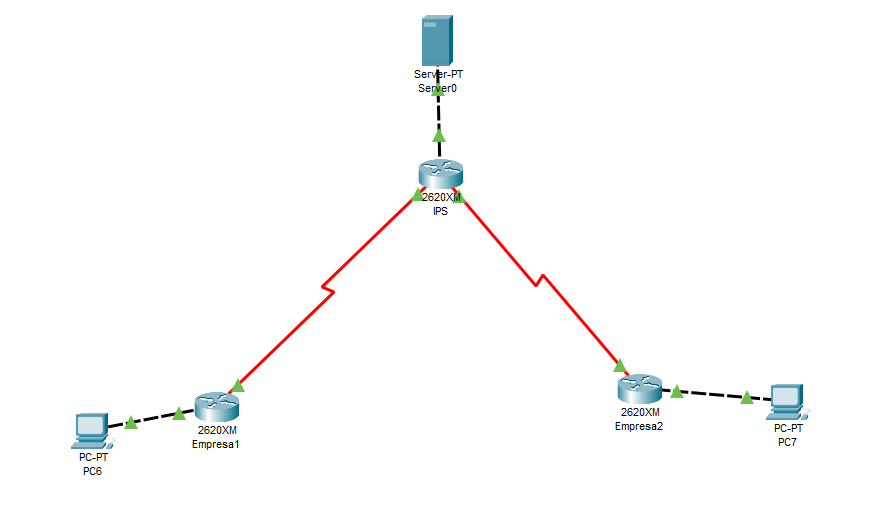
\includegraphics[width=0.7\textwidth]{img/Topologia.png}
        \caption{Topología}
        \label{fig:topologia}
    \end{figure}
    
    \subsection{Configuracion de los routers}
    En la siguiente imagen se puede apreciar la configuración del router que contiene el DTE, ya que está conectado a la red del servidor que aloja la página web. En este caso, el propósito es mostrar el servidor del proveedor de servicios de Internet.
    \begin{figure}[H]
        \centering
        \includegraphics[width=0.7\textwidth]{img/2.jpg}
        \caption{Imagen de Ejemplo}
        \label{fig:Imagen_Ejemplo2}
    \end{figure}
    En este caso, se puede observar la IP configurada en el puerto que se conecta al servidor. La IP del servidor es 10.0.0.10, por lo que la puerta de enlace es 10.0.0.1.
    En esta imagen se puede apreciar la otra parte de la configuracion del router DCE:
    \begin{figure}[H]
        \centering
        \includegraphics[width=0.8\textwidth]{img/5.jpg}
        \caption{Imagen de Ejemplo}
        \label{fig:Imagen_Ejemplo5}
    \end{figure}


    En la siguiente imagen se puede apreciar la configuración del router que contiene el DCE, ya que está conectado a la red del cliente que solicita la página web. En este caso, el propósito es mostrar el cliente que solicita la página web.
    \begin{figure}[H]
        \centering
        \includegraphics[width=0.8\textwidth]{img/3.jpg}
        \caption{Imagen de Ejemplo}
        \label{fig:Router DCE Empresa 1}
    \end{figure}

    \subsection{configuración de los protocolos}
    En la siguiente imagen se puede apreciar la configuración de los protocolos en el router que contiene el DCE. Se observa que solo se enrutan las redes públicas, mientras que en las redes privadas se utiliza NAT con su protocolo PAT, de manera que se pueda acceder al servidor del proveedor de servicios de Internet.
    
    \begin{figure}[H]
        \centering
        \includegraphics[width=0.8\textwidth]{img/4.jpg}
        \caption{Imagen de Ejemplo}
        \label{fig:NAT empresa 1}
    \end{figure}

    En esta imagen se puede apreciar la configuración del protocolo EIGRP para el proveedor de internet, en la cual se observa que se enrutan las redes públicas. Dado que no tenemos redes privadas, no es necesario enrutarlas.
    \begin{figure}[H]
        \centering
        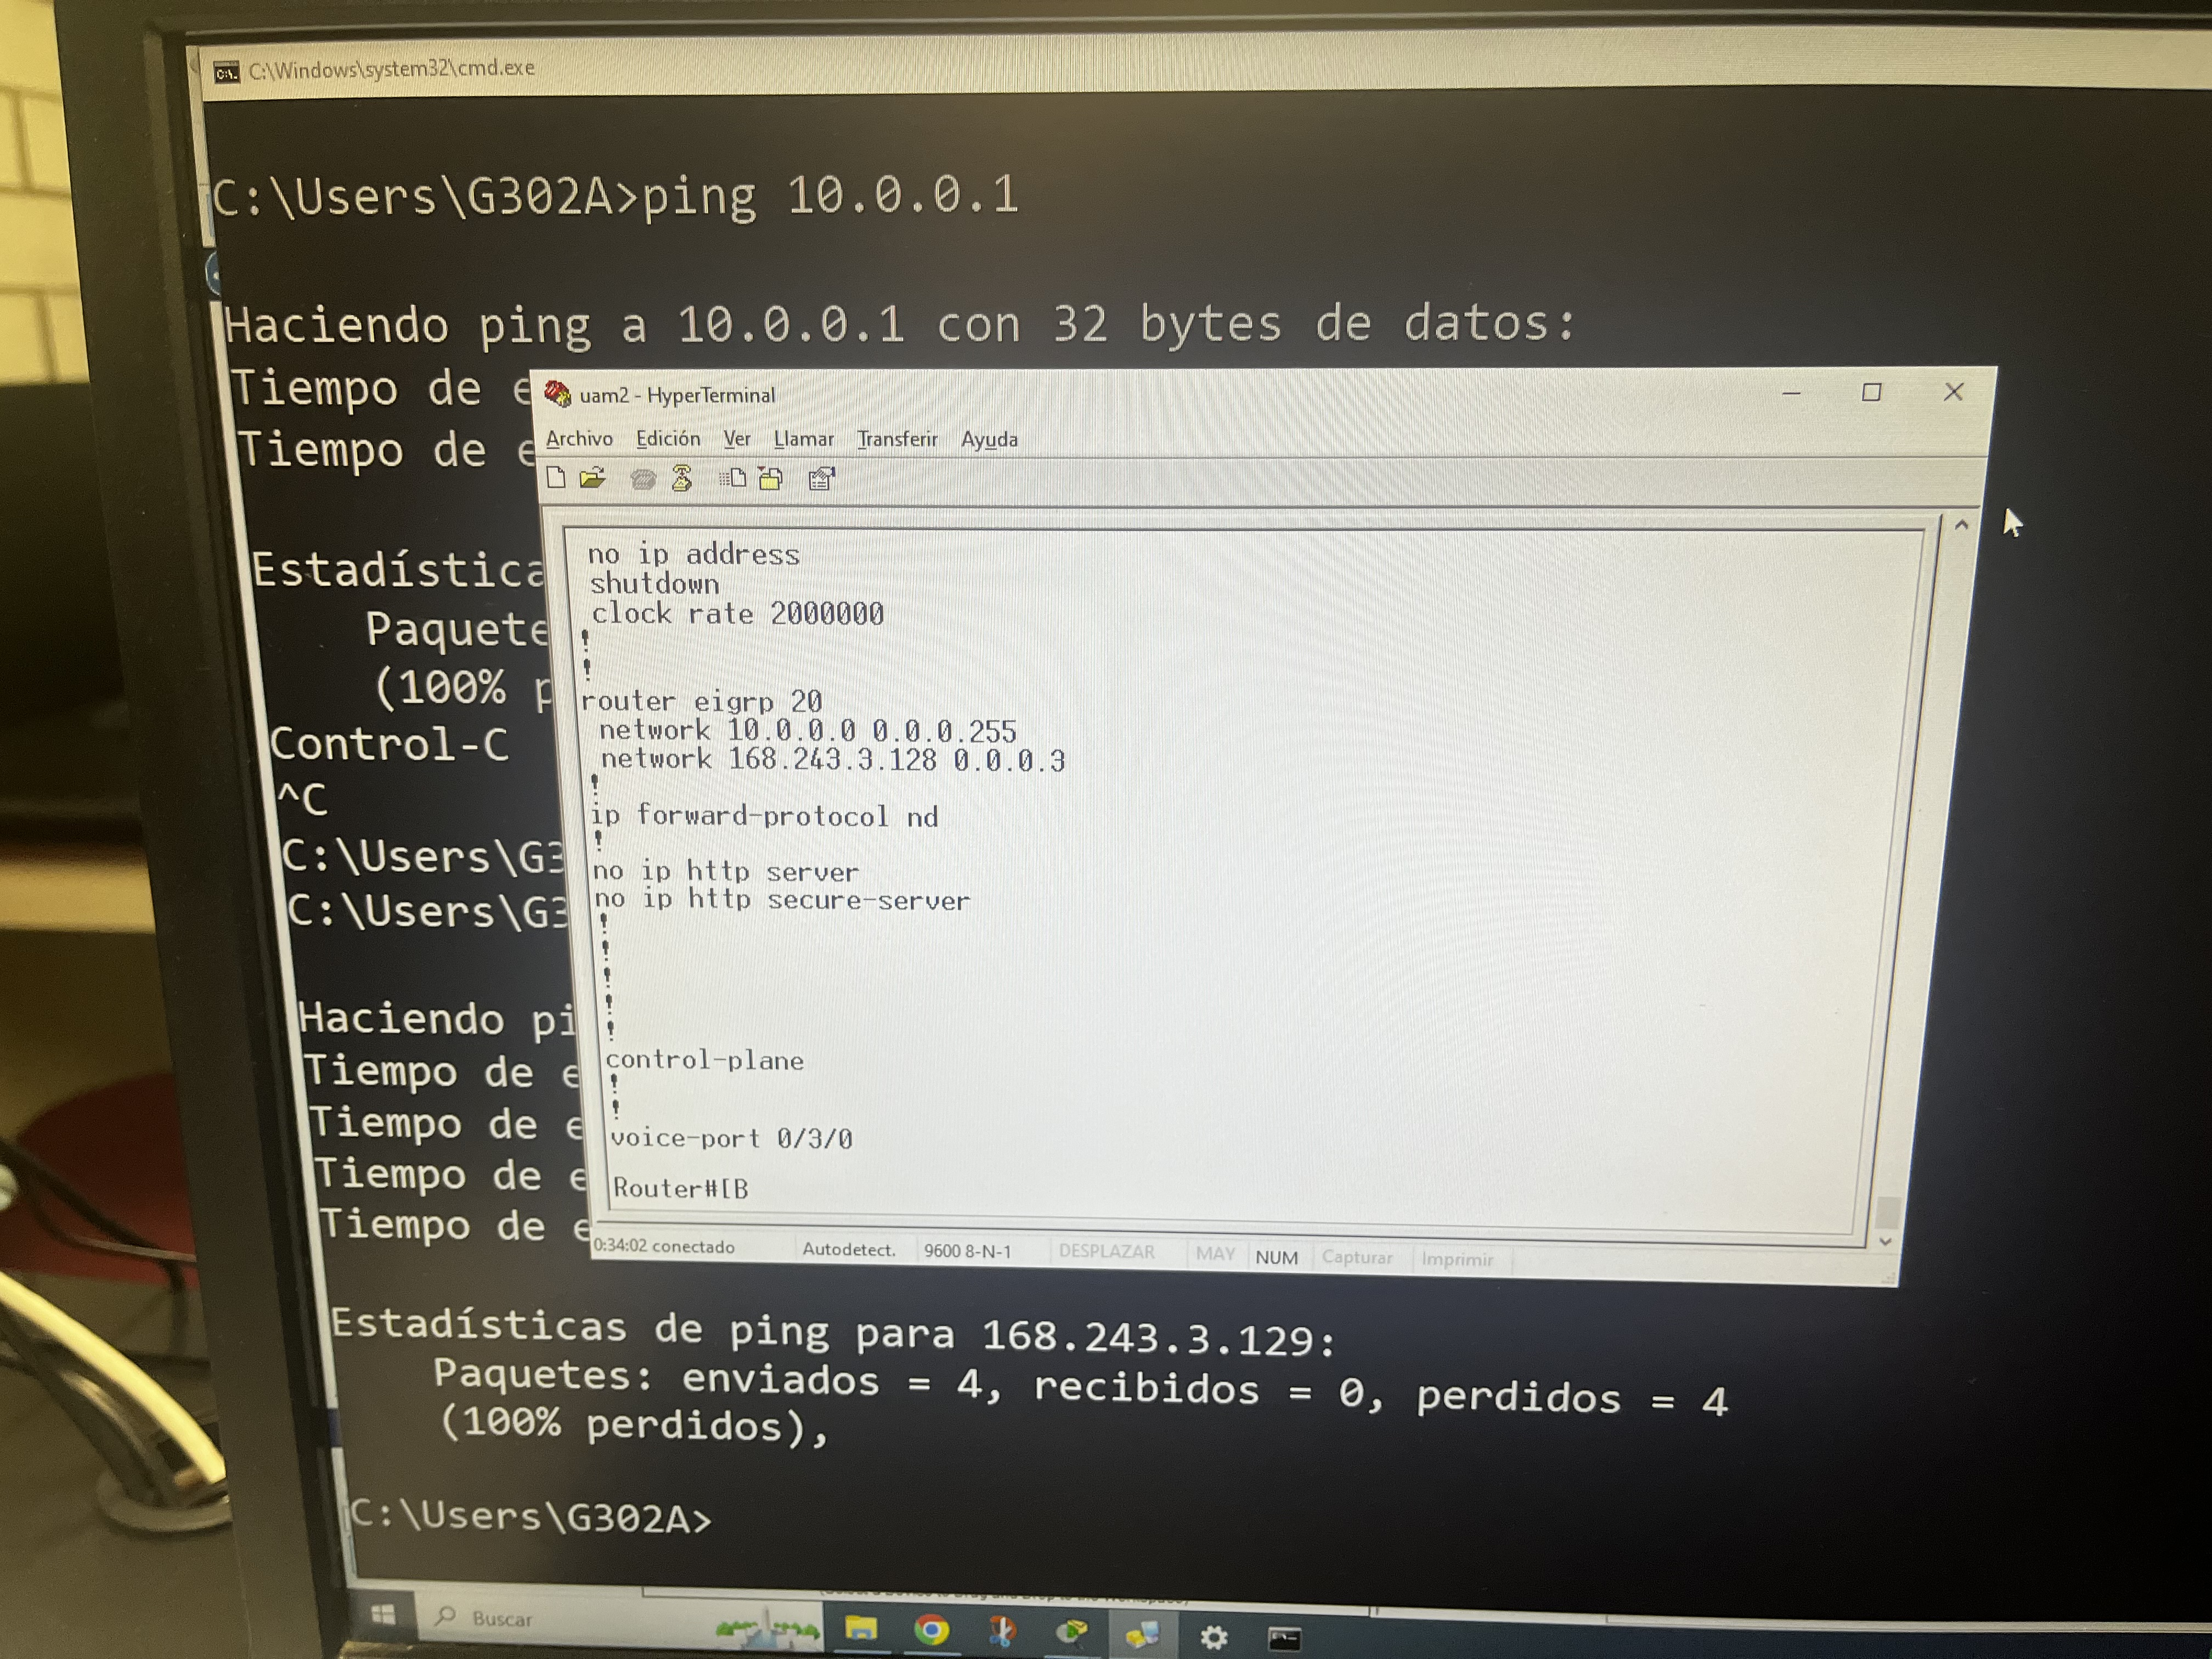
\includegraphics[width=0.8\textwidth]{img/6.jpg}
        \caption{Imagen de Ejemplo}
        \label{fig:EIGRP isp}
    \end{figure}
    En esta imagen podemos ver que se realizaron pruebas para la conexión al servidor del proveedor de servicios de Internet. Se puede observar que existe conexión y comunicación entre el cliente y el servidor mediante el comando ping.

    \begin{figure}[H]
        \centering
        \includegraphics[width=0.7\textwidth]{img/1.jpg}
        \caption{Imagen de Ejemplo}
        \label{fig:Imagen_Ejemplo1}
    \end{figure}

\section{Conclusiones}
Se puede concluir que, debido a la falta de tiempo, no fue posible completar correctamente la práctica del laboratorio asignada, por lo que no podemos emitir una evaluación sobre los resultados obtenidos. Sin embargo, todos los comandos y las imágenes presentadas corresponden a los realizados durante la práctica.

% --- Para agregar un apéndice
%\newpage
%\appendix
%\appendixpage
%\addappheadtotoc
%\section{Nombre del apéndice}